\documentclass[a4paper,11pt]{article}
\usepackage{biblatex}
\usepackage{graphicx}

\addbibresource{references.bib}
% pdflatex

% redefines the page margins
\setlength{\textheight}{24.00cm}
\setlength{\textwidth}{15.50cm}
\setlength{\topmargin}{0.35cm}
\setlength{\headheight}{0cm}
\setlength{\headsep}{0cm}
\setlength{\oddsidemargin}{0.25cm}

\title{\vspace{-2.0cm}%

\includegraphics{logoISEL}
D\'{A}DIVA IPO\\\large Digital Aid and Donor Information Verification Application for IPO
}

\author{
\begin{tabular}{c}
	Francisco Medeiros, No. 46631, e-mail: a46631@alunos.isel.pt, tel.: 913192828\\
	Luís Macário, No. 47671, e-mail: a47671@alunos.isel.pt, tel.: 933694131\\
	Ricardo Pinto, No. 47673, e-mail: a47673@alunos.isel.pt, tel.: 927111044\\
\end{tabular}}

\date{
\begin{tabular}{ll}
  {Supervisors:} & Filipe Freitas, e-mail: filipe.freitas@isel.pt \\
                 & João Pereira, e-mail: joaomiguel.pereira@cofidis.pt, Cofidis\\
\end{tabular}\\
\vspace{5mm}
\today}

\begin{document}

\maketitle

\tableofcontents

\section{Introduction}
Today, the professionals at the Instituto Português de Oncologia (IPO) in Lisbon, within the blood donor service, store and cross-check donor information in physical formats.

Currently, a donor arrives at the IPO and is asked to fill out and sign a paper pre-donation form. After filling out the form, the potential donor has a medical interview, where a doctor analyzes the form answers and asks additional questions to triage the donor's eligibility. If the donor has a pathology and/or is currently taking medication, this could be a cause for non-eligibility. Currently, the doctor has to look up all relevant information and determine implications in printed paper, which is a time-consuming and error-prone task.

This project aims to digitalize the pre-donation form and the medication and/or pathology interaction information. The reference information contained in this system must be easy to look up, update, and be customizable. The pre-donation form should be adaptable to the donor's answers.

The objective is to significantly decrease the possibilities of mistakes that storing/consulting information in a paper format brings and reduce the time it takes to donate blood by fast-tracking the signup and triage processes.

\section{System Requirements}

\subsection{Functional Requirements}
\begin{itemize}
	\item Donors should be able to quickly fill out a digital pre-donation form. The form should be adequate according to the current law, adaptable, and depend on the donor’s answers.
	
	\item Doctors should be able to find all relevant data on pathology and/or medication interactions with the donation in a digital format.
	
	\item Doctors and administrators should be able to access a back office used for customizing the pre-donation form and for updating the pathology and/or medication interaction information. The back office should also allow for user management.
	
	\item Google-like search and results by relevance - Search should be as simple as possible. There may be a need to increase the number of filters, but this complexity should be hidden. The results returned should be sorted based on relevance.
\end{itemize}

\subsection{Non-Functional Requirements}
\begin{itemize}
	\item Intuitive user experience through a simple and practical user interface.
	
	\item Responsive design that ensures a good user experience both on desktop and mobile.
	
	\item Complete and thorough documentation.
	
	\item Unit and integration testing with sufficient coverage to ensure confidence that the system is working without flaws.
	
	\item Good software engineering practices to ensure the fast development of the system.
\end{itemize}

\subsection{Optional Features}
\begin{itemize}
	\item After filling out the pre-donation form, the system could automatically check if the donor had any vaccinations and/or prescriptions that could be medically relevant. It would require integration with the IPO system, SNS, and/or Infarmed.
	\item The medical interview may be based on a pre-analysis, with the system having already identified possible risk vectors that better assist the doctor when deciding on accepting or refusing the donor.
	\item It can be possible to integrate with the already existing IPO system through the HL7 protocol. \cite{hl7}
	\item It is possible that the IPST has already implemented a digital system to maintain pathology and medication interaction information. If so, it would be possible to integrate this into our system, so that this information does not have to be manually updated.
	\item Users can authenticate using the Digital Mobile Key (CMD). It would require integration with the AMA (Administrative Modernization Agency) systems.
\end{itemize}

\section{Technologies}
We plan to use ASP.NET \cite{aspnet} to build the Web API, following DDD (Domain-Driven Design) and using the Minimal API \cite{minimalAPI} architecture. We will use Node.js \cite{nodejs} and React \cite{react} to deliver the front-end experience. We will use ElasticSearch \cite{elasticsearch} to store the donor’s data and the contextualized information. ElasticSearch will be used due to its searching capabilities, returning search results based on a relevance algorithm.

\section{Risks}
\begin{enumerate}
	\item C\# \cite{csharp} and ASP.NET are technologies that we’re not experienced in, resulting in some time being needed for adaptation.

	\item We are not experienced in building a UI/UX that has been deployed and used by end users. It could be a challenge to create an intuitive and engaging user interface that meets the expectations of our users.

	\item Difficulties defining the project scope, since the actual project depends on the IPO's needs.

	\item If we end up having to integrate into the existing software, that is something that we have not done, and it could present a challenge.
\end{enumerate}

\begin{figure}[h]
\centering
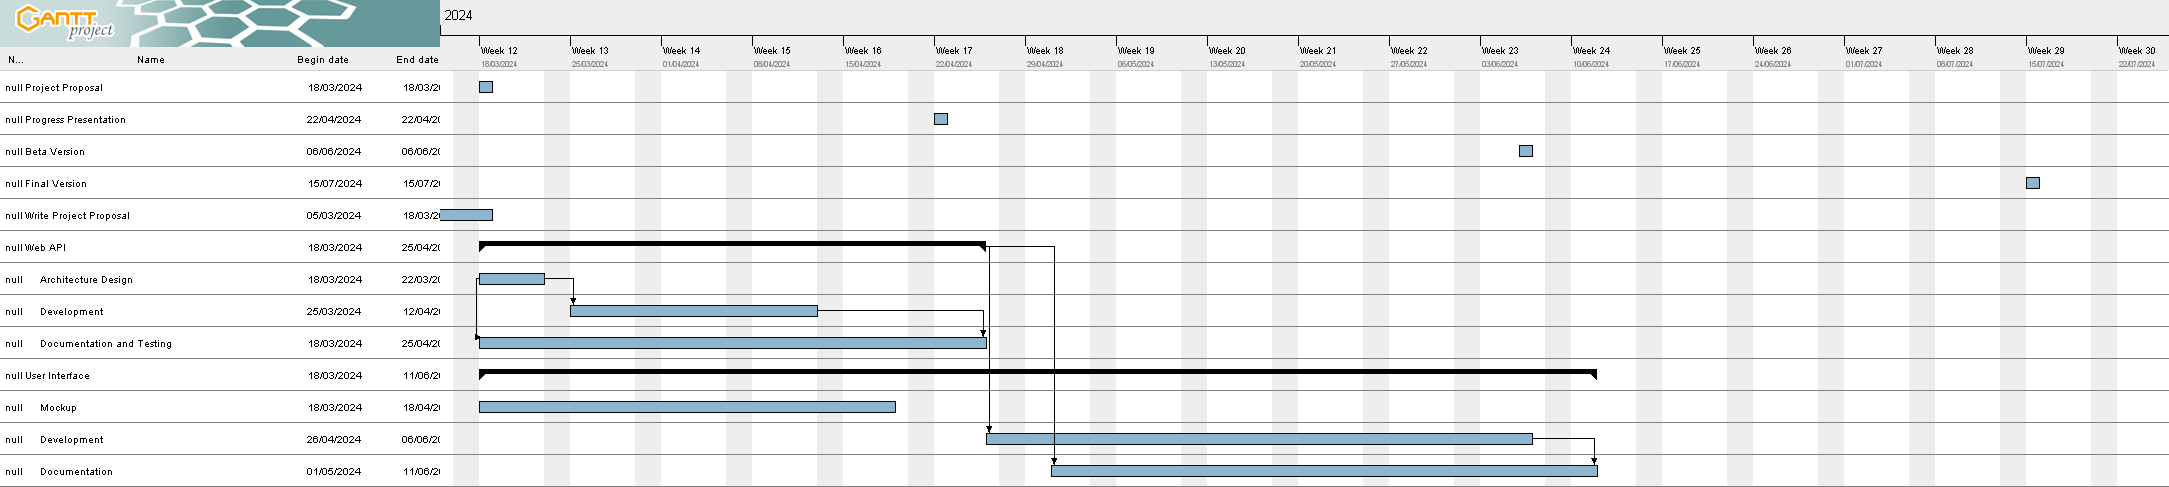
\includegraphics[width=\textwidth,height=\textheight,keepaspectratio]{gantt.png}
\caption{Provisory Gantt Chart}
\end{figure}

\section{Communication}
The project's scope is based on the specific needs of the IPO. To ensure the development process meets their expectations and follows the outlined plan, maintaining ongoing communication with the IPO is crucial.

The IPO will also assign a person to work alongside us throughout the project. This is designed not only to streamline communication between our team and the IPO, but also to ensure that the IPO has a knowledgeable point of contact who is familiar with our system's architecture and codebase. This is vital for ensuring the system can be maintained and updated after the project is completed, securing the long-term success of the project.

Within our team, we've established a weekly meeting between the students and the supervisors. This is designed to regularly assess the project's progress and address any concerns or adjustments needed to ensure its successful development.

\printbibliography[heading=bibintoc]

\end{document}